\documentclass{article}
%
%\usepackage{amsmath}
%\usepackage{amssymb}
%\usepackage{graphics}
%
\usepackage{graphicx}                              %for PNG images
\usepackage{color}                                 %for defining custom colors
\usepackage{framed}                                %for shaded and framed paragraphs
\usepackage{makeidx}                               %for index page
\usepackage{geometry}                              %for defining page size
\usepackage[linkbordercolor={0 0.8 0.8}]{hyperref} %for \url tag
\usepackage{doc}                                   %for pfill used by gist index style
%
\geometry{verbose,a4paper,tmargin=2.5cm,bmargin=2.5cm,lmargin=2.5cm,rmargin=2cm}
\makeindex
\hypersetup{
  pdfauthor = {Oxana Smirnova},
  pdftitle = {The Grid Monitor},
  pdfsubject = {Usage Manual},
  pdfkeywords = {Grid,NorduGrid,monitor,user,guide,reference,manual},
  pdfcreator = {PDFLaTeX with hyperref package},
  pdfproducer = {PDFLaTeX}
}
%
\usepackage[numbers]{natbib}
\bibliographystyle{plainnat}
%
\def\efill{\hfill\nopagebreak}%
\hyphenation{Nordu-Grid}
\setlength{\parindent}{0cm}
\setlength{\FrameRule}{1pt}
\setlength{\FrameSep}{8pt}
\addtolength{\parskip}{5pt}
\renewcommand{\thefootnote}{\fnsymbol{footnote}}
\renewcommand{\arraystretch}{1.3}
\newcommand{\dothis}{\colorbox{shadecolor}}
\definecolor{shadecolor}{rgb}{1,1,0.6}
\definecolor{salmon}{rgb}{1,0.9,1}
\definecolor{cyan}{rgb}{0,1,1}

\begin{document}
  \def\today{\number\day/\number\month/\number\year}
  
  \begin{titlepage}
    
    \begin{tabular}{rl}
      \resizebox*{3cm}{!}{
\includegraphics{ng-logo.png}}
      &\parbox[b]{2cm}{\textbf \it {\hspace*{-1.5cm}NORDUGRID\vspace*{0.5cm}}}
    \end{tabular}
    
    \hrulefill
    
    {\raggedleft NORDUGRID-MANUAL-5\par}
    
    {\raggedleft \today\par}
    
    \vspace*{2cm}
    
%%%%---- The title ----
    {\centering \textsc{\Large The Grid Monitor}\Large \par}
    
    \vspace*{0.5cm}
    
%%%%---- A subtitle, if necessary ----
    {\centering \textit{\large Usage manual}\large \par}
    
    \vspace*{2cm}
			
%%%%---- A list of authors ----
    {\centering \large Oxana Smirnova\footnote{O.Smirnova@cern.ch} \large \par}
    
    \vspace*{1.5cm}
    
%%%%---- An abstract ----
\begin{abstract}
  The Grid Monitor is a Web client tool for the ARC Information
  System, allowing to browse all the published information about the
  system. It makes use of the hierarchical information organization
  and the PHP LDAP module to provide a real-time monitoring and
  primary debugging for ARC-based grids.
\end{abstract}

\end{titlepage}
\thispagestyle{empty} $ $
\newpage
$\ $

\section{Introduction}
\label{sec:intro}

Information services play a very important role in any computational
grid architecture, being a nerve system of the Grid. Resource
discovery, scheduling, monitoring and many other tasks are impossible
without a reliable and up-to-date information about system components.

The MDS-inspired~\cite{mds} ARC Information
System~\cite{is} provides a robust and dynamic model for accessing not
only quasi-static information about resources and services, but also
about such rapidly changing parameters like queue and job
status. Being based on OpenLDAP~\cite{ldap}, it can be easily
interfaced to any browsing or monitoring tool, giving thus a
user-friendly overview of all the testbed resources.

The Grid Monitor makes use of the LDAP module of PHP~\cite{php} to
provide a Web client tool to browse the ARC information infrastructure. It
is available in many human languages\index{language} in order to follow browser
localization settings\footnote{In order to change the Monitor's language, simply
change the preferred language of your browser}. This
document gives a summary of its capabilities and usage guidelines.

\section{Grid Monitor Modules}
\label{sec:modules}

The structure of the Grid Monitor to great extent follows that of the
ARC Information System~\cite{is}. The basic objects are defined
by the following schema's objectclasses\index{objectclass}:
\begin{list}{--}{\itemsep=-0.5mm}
\item \textsf{nordugrid-cluster}: a cluster \index{nordugrid-cluster}
\item \textsf{nordugrid-queue}: a queue at the cluster, accessible by
  the authorised users \index{nordugrid-queue}
\item \textsf{nordugrid-job}: a Grid job, associated with a queue
  \index{nordugrid-job}
\item \textsf{nordugrid-authuser}: a user, authorized to submit jobs
  to a given queue \index{nordugrid-authuser}
\end{list}

The Grid Monitor also uses the Virtual Organisation (VO)
\textsf{organisationalPerson} and Storage Element
\textsf{nordugrid-se} objectclasses, and their attributes.

For each objectclass, either an essential subset of attributes, or the
whole list of them, is presented in an easily accessible inter-linked
manner. This is realized as a set of browser windows, each being associated
with a corresponding module. There are nine major modules
\index{modules}: \newcounter{count1}
\begin{list}{\arabic{count1})}{\usecounter{count1} \itemsep=-0.5mm}
\item An overall Grid Monitor
\item Cluster Description
\item Queue Details
\item Job Information
\item User Information
\item Attributes Overview
\item Customizeable Display Tool (``Match-it-yourself'')
\item List of Storage Facilities
\item List of Users
\end{list}
Each module displays both dynamic and static information: for example,
a queue name is static, while the amount of running jobs in this queue
is dynamic. Most of the displayed objects are linked to appropriate
modules, such that with a simple mouse click, a user can launch
another module, expanding the information about the corresponding
object or attribute. Each such module opens in an own window, and
gives access to other modules in turn, providing thus a rather
intuitive browsing.

In what follows, these modules are described in details, giving an
overview of their functionality and usage hints.

\subsection{The Grid Monitor}
\label{sec:loadmon}

The basic module, \index{grid monitor} providing access to the most
required information, is the Grid Monitor, showing the overall status
of the system. It serves as a starting point for browsing the system
information. The purpose of this module is to give a quick overview of
the current status of the Grid infrastructure by showing the list of the
available clusters and the most essential information about them: an
alias, number of working processors, number of occupied processors and
number of queueing jobs. In the current implementation, the main Grid
Monitor window contains also the link to the user base of the infrastructure. 
Figure~\ref{fig:loadmon} shows a screenshot of the running
monitor. All the information shown is dynamic, including
organizational names (countries in this case).

\begin{figure}[ht]
\centering{{\scalebox{0.9}{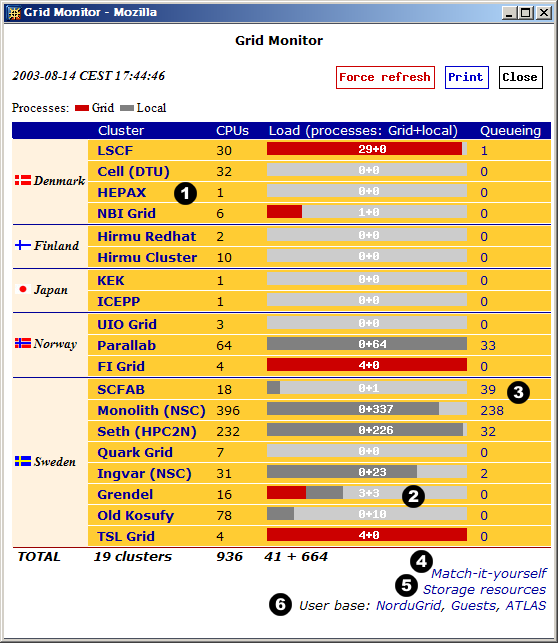
\includegraphics{loadmon.png}}}
\caption{\label{fig:loadmon}The Grid Monitor} }
\end{figure}

In Figure~\ref{fig:loadmon}, the numbered tags indicate clickable
objects as explained below:
\newcounter{count2}
\begin{list}{\arabic{count2})}{\usecounter{count2} \itemsep=-0.5mm}
\item \textsf{Cluster}: a cluster alias, \index{cluster>alias} linked
  to the cluster description module (Section~\ref{sec:clusdes}), which
  provides complete information about the current status of a cluster.
\item \textsf{Load}: a graphical and numeric representation of the
  cluster load, \index{cluster>load} showing both Grid- and non-Grid
  (submitted locally) running processes. Colored bar shows percentage of
  Grid processes, while the grey bar shows total relative
  occupancy of a cluster. Numbers indicate the absolute amount of
  running processes, with first figure corresponding to the Grid, and
  second - to the non-Grid ones. It should be noted that number of
  processes does not necessarily correspond to the number of running
  jobs: a parallel job \index{job>parallel} can occupy several
  processors. By clicking on a bar, a user accesses the list of all
  Grid jobs, \index{job>running} running on a cluster
  (Section~\ref{sec:jobstat}).
\item \textsf{Queueing}: number of queueing jobs, \index{job>queueing}
  which includes both jobs queued in an LRMS and those being
  pre-processed by the Grid Manager~\cite{gm}. Only jobs which can be
  potentially executed in a Grid queue are counted. The number is
  linked to the same module as the \textsf{Load} item, with the only
  difference that it displays the list of the Grid-queued jobs. Note
  that non-Grid jobs are counted in the total number of queued jobs,
  while they can not be listed by the Grid Monitor, as they are not
  providing any information in the ARC Information System.
\item \textsf{Match-it-yourself}: link to the ``Match-it-yourself''
  interface (Section~\ref{sec:match}) which allows users to compose
  non-standard monitor requests. \index{Match-it-yourself}
\item \textsf{Storage resources}: link to the list of available
  storage resources (Section~\ref{sec:storage}). \index{storage}
\item \textsf{User base}: several auxiliary links, providing an access
  to the VO-listing module (Section~\ref{sec:vo-users}). The main
  purpose of this link is to provide an easy access to the
  user-specific information, such as the list of submitted jobs and
  available resources.
\end{list}

\subsection{Cluster Description}
\label{sec:clusdes}

The cluster description \index{cluster} module displays all the
cluster attributes stored in the local information tree, as well as most
relevant
information about the queues, accessible by the Grid users. The
window thus contains two lists, as shown in Figure~\ref{fig:clusdes}:

\newcounter{count3}
\begin{list}{\arabic{count3})}{\usecounter{count3} \itemsep=-0.5mm}
\item \textsf{Attributes}: \index{cluster>attributes} this is a dump
  of all the attributes of the \textsf{nordugrid-cluster} objectclass,
  dynamic and static ones. Such attributes as cluster alias, or domain
  name, are static; others are dynamic, with the values obtained by
  the information providers: e.g., total CPU number,
  amount of jobs, or available disk space. More details about these
  attributes can be found in the ARC Information System
  description~\cite{is}. Each attribute (apart of the time stamps)
  is linked to the Attributes Overview module
  (Section~\ref{sec:attlist}), such that clicking on an attribute name
  brings the list of the values of this particular attribute on all
  the Grid clusters. For instance, this is the most convenient
  way to browse available disk space \index{disk space} or runtime
  environment\index{runtime environment} values over the system.
\item \textsf{Queues}: \index{queue>list} the list of queues at a
  given cluster, accessible by the Grid users. While the detailed
  list of queue attributes and corresponding jobs can be obtained by
  clicking on a queue name (see Queue Details module description,
  Section~\ref{sec:quelist}), the most essential parameters are listed
  already in the Cluster Description module. They are: queue name,
  \index{queue>name} queue status, queue length \index{queue>length}
  (minimal and maximal), number of CPUs assigned to a queue (if
  available), and number of running and queued jobs. Since queues can
  be shared between Grid and local users, the total number of jobs is
  shown, with the number of Grid jobs in parentheses.
\end{list}

The Cluster Description module is linked from most other modules (except
the List of Users one): clicking on a domain name of a cluster brings
the Cluster Description window.

\begin{figure}[ht]
\centering{
{\scalebox{0.6}{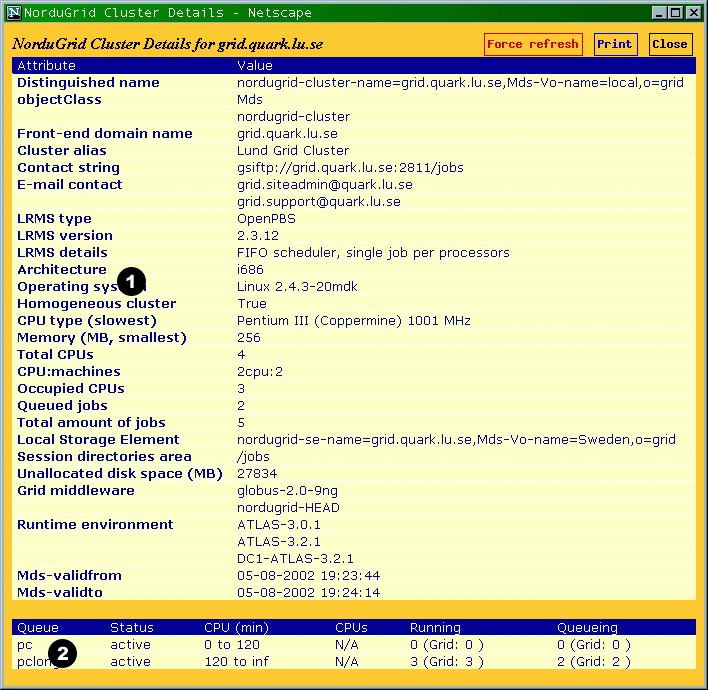
\includegraphics{clusdes.jpg}}}
\caption{\label{fig:clusdes}Grid cluster details} }
\end{figure}

\subsection{Queue Details}
\label{sec:quelist}

In the ARC Information System, \index{queue} the
\textsf{nordugrid-queue} objectclass is described by a set of
queue-specific attributes, and has two sub-trees: \textsf{nordugrid-job}
and \index{job} \textsf{nordugrid-authuser}. This structure reflects the
fact that users are not implicitly authorized to submit jobs to any
queue. However, the list of users allowed to a specific queue is a
fairly static information, and thus is beyond the scope of the Grid
Monitor\footnote{List of queues available for a given user can be
obtained through the User Information module}.

\begin{figure}[ht]
\centering{
{\scalebox{0.32}{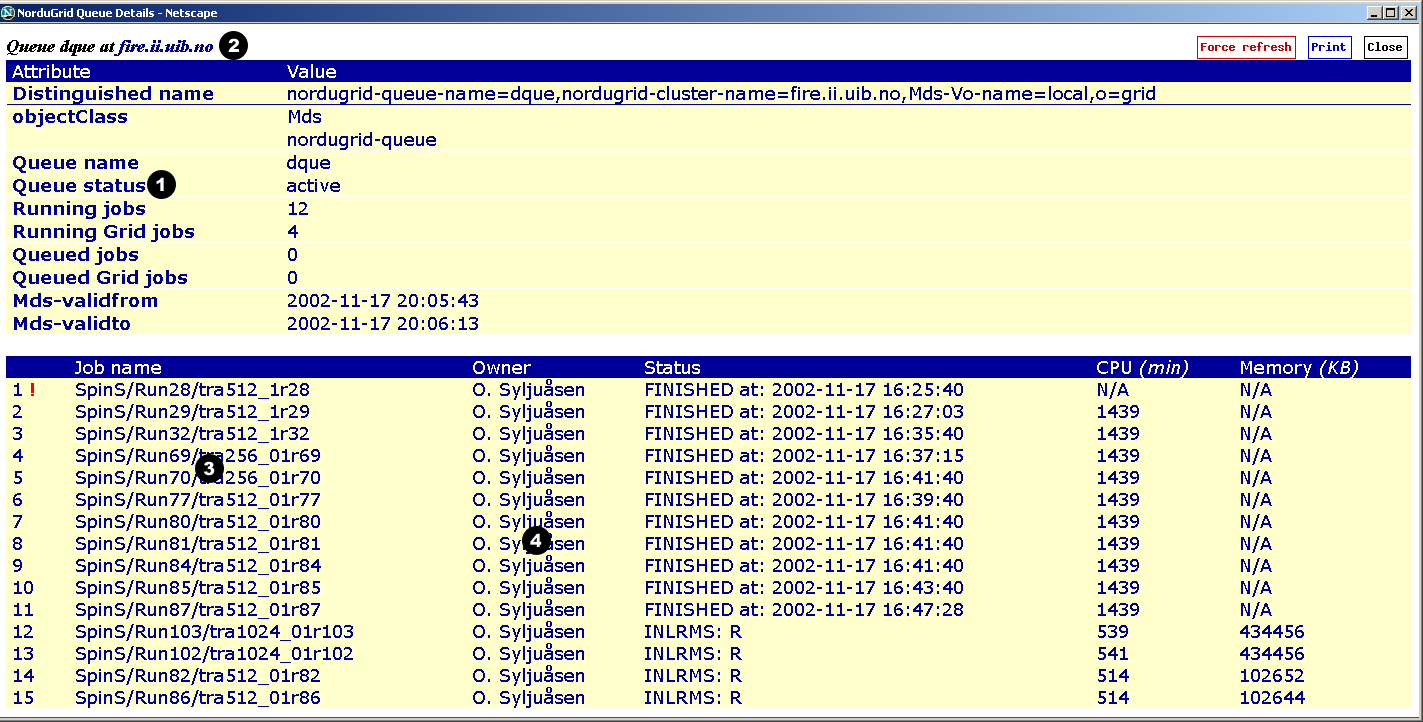
\includegraphics{quelist.png}}} }
\caption{\label{fig:quelist}Grid queue details}
\end{figure}

The Queue Details module provides the list of the queue attributes and
of all the jobs scheduled (running or waiting) to this queue.
Figure~\ref{fig:quelist} shows the queue description window,
with clickable fields marked by numbered tags as follows:

\newcounter{count4}
\begin{list}{\arabic{count4})}{\usecounter{count4} \itemsep=-0.5mm}
\item \textsf{Attributes}: \index{queue>attributes} the dump of the
  queue attributes. Just like the cluster attributes
  (Section~\ref{sec:clusdes}), they can be both static and
  dynamic. Every attribute is linked to the Attributes Overview module
  (Section~\ref{sec:attlist}), which allows to browse the values of
  each attribute over all the Grid system.
\item \textsf{Cluster name}: each queue is associated with the
  cluster, which name is shown at the top of the window. Clicking the
  cluster name brings up the Cluster Description window
  (Section~\ref{sec:clusdes}).
\item \textsf{Job name}: from the Queue Details window, users can get
  access to detailed information about every job \index{job>in a
  queue} in the queue by clicking the job name.\index{job>name} Each
  job name is linked to the Job Information module, described in
  Section~\ref{sec:jobstat}.
\item \textsf{Owner}: \index{job>owner} The Grid authentication
  mechanism allows to associate every job with a corresponding user,
  even though an actual Unix account owner may be a generic
  "griduser". The Grid Monitor uses this feature to display explicitly
  each job owner. In the Queue Details window (as in all other
  modules), user's name is linked to the User Information module
  (Section~\ref{sec:userlist}), which displays all the resources
  available for a given user, as well as the list of user's jobs.
\end{list}

Queue Information module is accessible via links to queue names in the
Cluster Information (Section~\ref{sec:clusdes}), Job Information
(Section~\ref{sec:jobstat}), User Information
(Section~\ref{sec:userlist}) and Attributes Overview
(Sec~\ref{sec:attlist}) modules.

\subsection{Job Information}
\label{sec:jobstat}

The Job Information module is activated on three different occasions:
\begin{list}{--}{\itemsep=-0.5mm}
\item To display a list of all running Grid jobs
  \index{job>running} on a cluster
\item To display a list of all queued \index{job>queued} Grid
  jobs on a cluster
\item To show the full information on a given job
\end{list}

Lists of running and queued jobs \index{job>{on cluster}} are
accessible from the top Grid Monitor window
(Section~\ref{sec:loadmon}) by clicking the corresponding fields
(marked 2 and 3 in Figure~\ref{fig:loadmon}).  As shown in
Figure~\ref{fig:jobstat2}, such a list contains not only job names,
but also their respective owners, status (as returned by the Grid
Manager), execution time (in case of running jobs), and the submission
queue.

\begin{figure}[hb]
\centering{
{\scalebox{0.4}{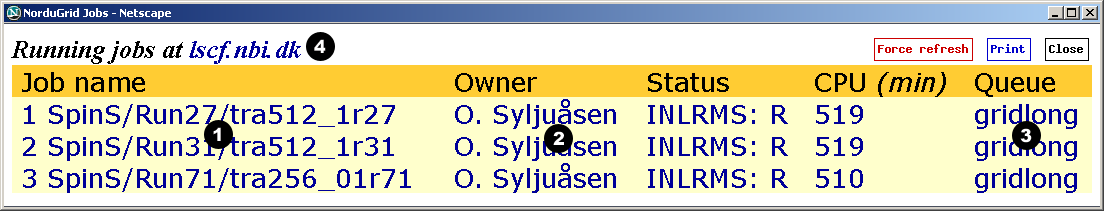
\includegraphics{jobstat2.png}}} }
\caption{\label{fig:jobstat2}Grid job list}
\end{figure}

Most of the fields in a job list window are linked to the corresponding
monitor modules, giving access to more detailed information:
\newcounter{count5}
\begin{list}{\arabic{count5})}{\usecounter{count5} \itemsep=-0.5mm}
\item \textsf{Job name}: just like in the Queue Details window
  (Section~\ref{sec:quelist}), the job name is linked to the Job
  Information window, described below. However, while the Queue
  Details module lists the jobs in a given queue, the Job Information
  window gives an overview of all the Grid jobs on a cluster.
\item \textsf{Owner}: this field is also identical to the one in the
  Queue Details window: user's name is linked to the User Information
  module (Section~\ref{sec:userlist}), which displays all the
  resources available for a given user and the list of user's jobs.
\item \textsf{Queue}: the name of the queue is liked to the Queue
  Details window (Section~\ref{sec:quelist}), which gives a snapshot
  of the queue status, including al the Grid jobs submitted to a
  particular queue -- running or waiting.
\item \textsf{Cluster name}: clicking on the cluster name brings up
  the Cluster Description window (Section~\ref{sec:clusdes}), which
  gives a general overview of a given cluster and the status of its
  queues (those available for the Grid users).
\end{list}

\begin{figure}
\centering{
{\scalebox{0.6}{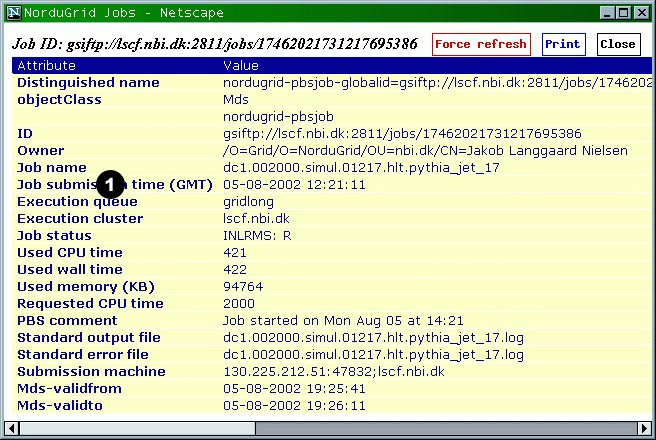
\includegraphics{jobstat1.jpg}}} }
\caption{\label{fig:jobstat1}Grid job statistics}
\end{figure}

The job \index{job>information} information window is invoked by
clicking on a job name in any Grid Monitor window which lists jobs. It
is handled by the same module which produces running/queued job list,
and contains simple dump of all the available job attributes (see
Figure~\ref{fig:jobstat1}). Just like in the Cluster Description and
Queue Description windows, each attribute is clickable (as indicated
by a tag numbered 1 in Figure~\ref{fig:jobstat1}), and is linked to
the Attributes Overview module (Section~\ref{sec:attlist}). This is a
convenient way to compare jobs that reside on the system.

\subsection{User Information}
\label{sec:userlist}

The User Information \index{user information} module of the Grid
Monitor gives access to all the available information, related to a
given user. This includes the list of available resources
\index{resources} (queues, processors and disk space), and the list of
user jobs, residing on the system at the time of query. To collect
this information, the whole system has to be queried, therefore
invocation of this module typically takes quite a bit of time (at
least comparing to most other modules).

\begin{figure}
\centering{
{\scalebox{0.4}{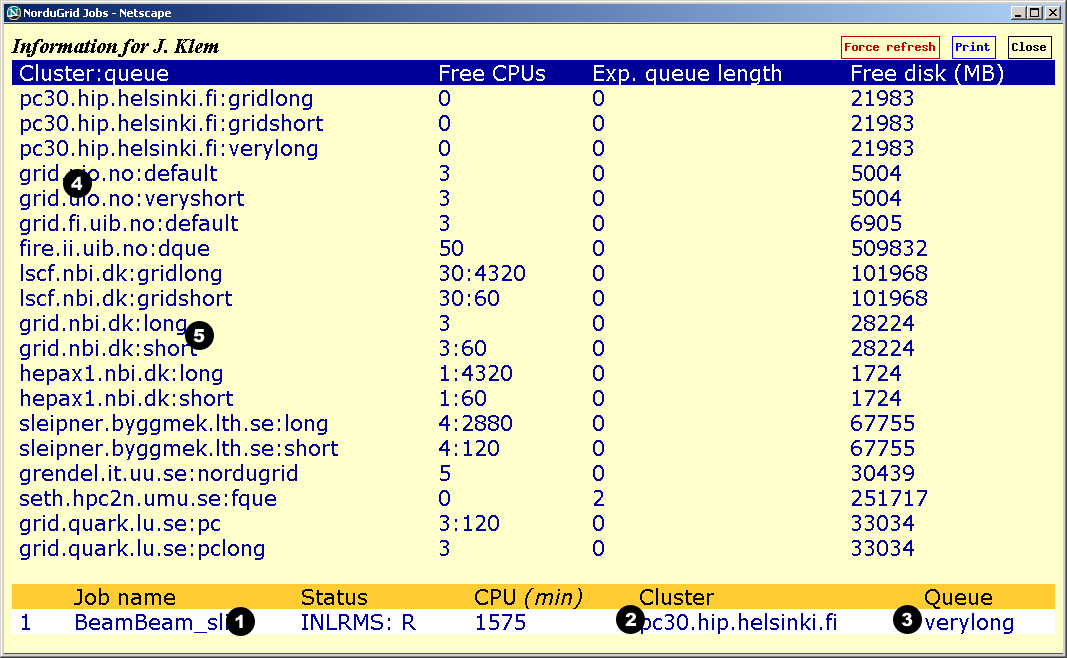
\includegraphics{userlist.png}}} }
\caption{\label{fig:userlist}Grid user information}
\end{figure}

Figure~\ref{fig:userlist} shows a typical User Information window, where
the numbered fields are linked to other Grid Monitor modules:
\newcounter{count6}
\begin{list}{\arabic{count6})}{\usecounter{count6} \itemsep=-0.5mm}
\item \textsf{Job name}: \index{job>by user} this field is linked to
  the Job Information window (Section~\ref{sec:jobstat}), providing
  access to the detailed information on a given job. Unlike of Job
  Information or Queue Information modules, which list local to a
  cluster jobs, the User Information module collects all the jobs
  submitted by a given user to the whole system.
\item \textsf{Cluster}: since the User Information window displays all
  the jobs associated with a given user, description of each
  respective cluster is available by clicking the cluster name. This
  brings up a cluster description window, described in
  Section~\ref{sec:clusdes}.
\item \textsf{Queue}: this field is linked to the Queue Details module
  (Section~\ref{sec:quelist}), thus giving access to the information
  about the status of the relevant queue.
\item \textsf{Cluster}: the upper part of the User Information window
  lists the Grid resources, available for a user. Each cluster,
  to which a user is authorized to submit jobs, is indicated by its
  name.  Cluster names are linked to the Cluster Description window
  (Section~\ref{sec:clusdes}), giving detailed information on
  available resources.
\item \textsf{Queue}: since users authorization may be not only
  cluster-based, but also queue-based, the allowed queue information
  can be accessed by clicking a queue name. This brings up the Queue
  Details window, described in Section~\ref{sec:quelist}.
\end{list}

The simplest way to access the User Information window is via the List
of Users (Section~\ref{sec:vo-users}), although it can be invoked from
any Grid Monitor window where a user name is displayed (e.g., a Job
Information or a Queue Details window).

\subsection{Attributes Overview}
\label{sec:attlist}

As it was mentioned above, every ARC objectclass attribute,
\index{attributes} appearing in a Grid Monitor window, is linked to
the Attributes Overview module, which queries all the relevant objects
on the system and delivers a comparative list of the
attributes. Similarly to the User Information module, querying all the
Grid resources takes somewhat long time, as the Grid Monitor does
not have an own cache.

This module can also be accessed via the ``Match-it-yourself''
interface (Section~\ref{sec:match}). In this case, it can list as many
attributes as specified by a user request, eventualy applying the user
selection criteria.

\begin{figure}[hb]
  \centering{
    {\scalebox{0.6}{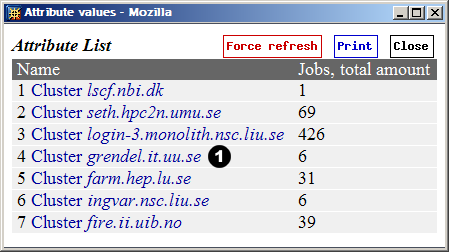
\includegraphics{attlist.png}}} }
  \caption{\label{fig:attlist}Grid objects grouped by attribute}
\end{figure}

Figure~\ref{fig:attlist} shows a typical result of the Attributes
Overview query: in this example, the \textsf{nordugrid-cluster}
attribute "Jobs, total amount" was queried, and a comparative list of
results returned. The \textsf{Resource} field (indicated by the tag 1)
depends on the nature of the attribute, and can be either of:
\begin{list}{--}{\itemsep=-0.5mm}
\item cluster name, linked to the Cluster Description module,
\item cluster name and queue name, linked to the Cluster Description
  and Queue Details modules respectively,
\item job ID string (see ref.\cite{gm} for details), linked to the Job
  Information module.
\end{list}

\subsection{``Match-it-yourself''}
\label{sec:match}

The ``Match-it-yourself'' \index{Match it yourself} is a customizeable
interface to the Attributes Overview module
(Section~\ref{sec:attlist}). It allows users to chose which attributes
of an object to display, optionally applying filters. While the other
Monitor windows display a pre-defined set of data, this module gives
an advanced user a possibility to build a customized request to the
Information System.

An example use case for this interface could be a user desiring to
view a list of his running (but not queued or finished) jobs, complete
with used CPU and wall time, memory and job name. The
``Match-it-yourself'' tool would be then invoked for the \textsf{job}
object, and the display request would contain \textsf{Name},
\textsf{Used CPU time}, \textsf{Used wall time}, \textsf{Used memory
  (KB)}, and \textsf{Status} -- the latter with a filter
\fbox{\textsf{Status = INLRMS: R}}.

\begin{figure}[ht]
  \centering{
    {\scalebox{0.6}{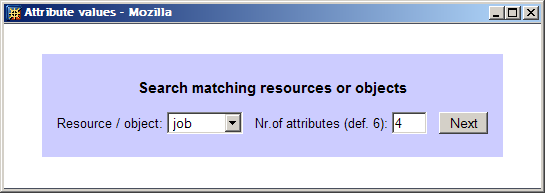
\includegraphics{match1.png}}} }
  \caption{\label{fig:match1}Object class selection window}
\end{figure}

Figure~\ref{fig:match1} shows the first screen of the
``Match-it-yourself'' interface, which welcomes users to select the
object class to work with, and the amount of attributes to be
displayed. When not sure about the latter, users should specify a top
estimate -- unused fields will be ignored in further searches.

\begin{figure}[hb]
  \centering{
    {\scalebox{0.6}{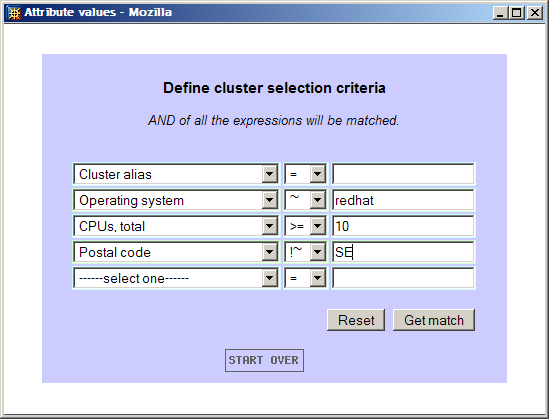
\includegraphics{match2.png}}} }
  \caption{\label{fig:match2}Attribute selection window}
\end{figure}

Figure~\ref{fig:match2} is a snapshot of the screen where the
atttributes to display and their selection criteria are specified. If
a user wishes to display an attribute for all the objects,
independently of its value, the rightmost field may be either kept
empty, or filled with an asterisk (\verb#*#), while the middle field
should be set to ``$=$''. Whenever a filter has to be applied, an
operator should be selected in the middle column, and a match string
specified in the rightmost field. For example, if only clusters
containing ``NBI'' in their domain names have to be shown, the
attribute filter would be \fbox{\textsf{Front-end domain name $\sim$
nbi}}. Matches are case-insensitive.

 \begin{figure}[ht]
   \centering{
     {\scalebox{0.6}{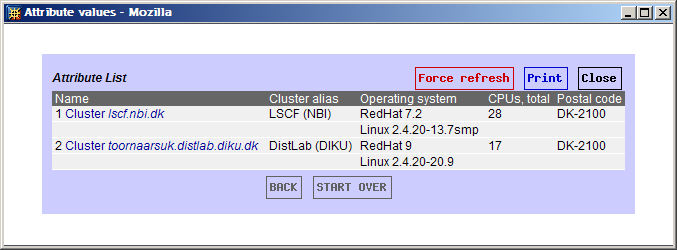
\includegraphics{match3.png}}} }
   \caption{\label{fig:match3}Customized cluster information display}
 \end{figure}

Figure~\ref{fig:match3} is the result of the search according to the
criteria defined in the exampel in Figure~\ref{fig:match2}. Three
filters were applied: on operating system attribute, total number of
CPUs and postal code (in this case we were selecting any cluster which
is not in Sweden). Since we wanted to display each cluster's alias as
well, this attribute was added to the selection, but with a ``match
everything'' scope. The attribute matching method is exactly the same
as used by the Attributes Overview module (Section~\ref{sec:attlist}),
and it re-uses the screen layout shown in Figure~\ref{fig:attlist}.

\subsection{Storage Resources}
\label{sec:storage}

\index{Storage resources}Although there is no well-defined Storage
Element\index{Storage Element} concept in ARC, some
information about the storage resources can be found in the
Information System. The Storage Resources module, linked from the main
Monitor window, displays all the available information for those
Storage Elements which publish it. Particularly important is the base
URL, which specifies the Grid mount point that could be used in job
descriptions.

\begin{figure}[hb]
  \centering{
    {\scalebox{0.7}{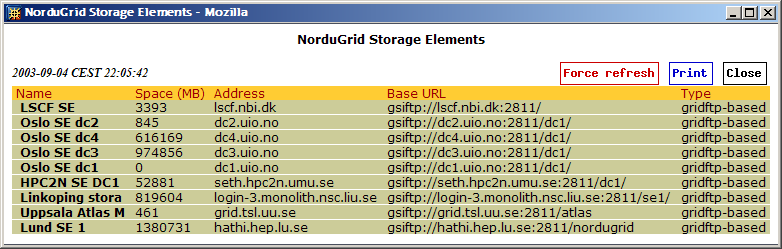
\includegraphics{storage.png}}} }
  \caption{\label{fig:storage}List of storage elements}
\end{figure}

\subsection{List of Users}
\label{sec:vo-users}

The List of Users \index{user list} module is different from the rest
of the Grid Monitor modules because it does not deal with the
ARC information system. Instead, it retrieves lists of users from
VO databases~\cite{vo}. It serves as a link between different databases
(LDAP and VO), by interfacing each user record to the User Information
module (Section~\ref{sec:userlist}). Figure~\ref{fig:vo-users} shows a
screenshot of a typical VO user list, with numbered tags indicating
clickable links as follows: \newcounter{count7}
\begin{list}{\arabic{count7})}{\usecounter{count7} \itemsep=-0.5mm}
\item \textsf{Name}: user name as given in the corresponding Grid
  certificate field, linked to the User Information module
  (Section~\ref{sec:userlist}).
\item \textsf{E-mail}: E-mail \index{E-mail} address of a user, if
  available. It is linked to an e-mail URL, allowing to send a message
  to a user directly from the browser (if such an option is enabled in
  a browser).
\end{list}

\begin{figure}[ht]
  \centering{
    {\scalebox{0.6}{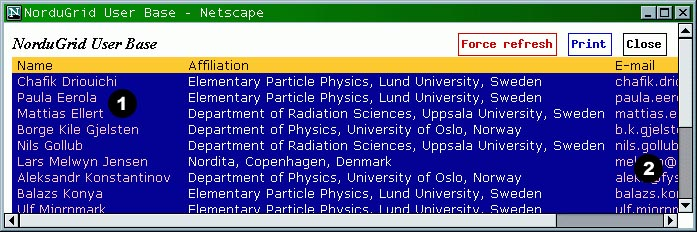
\includegraphics{vo-users.jpg}}} }
  \caption{\label{fig:vo-users}List of the Grid users}
\end{figure}

The List of Users is available only from the top Grid Monitor window.

\section{Implementation notes}
\label{sec:implement}

The Grid Monitor is implemented entirely in PHP, with optional usage
of client-side JavaScript. Since all the databases the Grid Monitor
has to deal with are hierarchical LDAP ones, the server-side LDAP
module of PHP is absolutely necessary to be enabled in order to make
the Grid Monitor functioning. The PHP LDAP module conveniently allows
parallel LDAP searches, -- the feature heavily used by the Grid
Monitor, since it speeds up the data retrieval.

The Grid Monitor uses only minimal disk caching (overview window only), storing
all the LDAP
query results in the memory. To minimize the memory usage, only the
attributes relevant to each query are retrieved.

In order to speed up the queries, the Grid Monitor makes as little use
of the original MDS information propagation mechanisms as possible. GIIS and
GRIS services are used only as link collections\footnote{Globus MDS2.2
provided a quick access to the lower level servers via a base scope
LDAP search for the "giisregistrationstatus" attribute}.

Since the ARC architecture makes use of several equivalent
top-level GIIS servers, the Grid Monitor queries all of them in order
to have a reliable access to all the system information. In some
cases, lower-level GRIS servers can also be duplicated, hence the Grid
Monitor contains a built-in mechanism to prevent
double-counting.

Discovery of lower-level GRIS servers is done recursively, starting
from the registration information in all the top-level indexes, and
ending at the local level. This recursive search method is invoked not
only to discover clusters in e.g., the main Monitor module, but also
to locate storage facilities.

All the Grid Monitor windows are automatically refreshed by the means
of the built-in browser HTML instructions. Every window can be
forcefully refreshed, printed and closed by using either standard
browser tools, or the provided JavaScript-enabled buttons.

In the top Grid Monitor window, clusters are automatically grouped by
respective second-level hierarchy VOs -- in the described above
case, this is nothing but countries.

Such fields as cluster aliases, user names and attribute names, are
customizable, and can be adjusted from the stored in the information system
values to
any more appropriate ones, depending on the actual requirements.

In general, the Grid Monitor was designed to be a cross-browser,
cross-platform tool, and have been shown to work properly with browsers
\index{browsers} ranging from Lynx to Konqueror to Microsoft Internet
Explorer.

%% \section{HOWTO}
%% \label{sec:howto}

%% This is a list of most common examples of the Grid Monitor usage.

%% \begin{description}
%% \item[How to list all the jobs submitted by a user?]$\ $\\ Click a
%%   user name in any window, e.g., in the List of Users
%%   (Figure~\ref{fig:vo-users}, item 1). The List of Users is available
%%   from the top Grid Monitor window (Figure~\ref{fig:loadmon}, item 4).
%% \item[Why the jobs finished two days ago do not show up?]$\ $\\
%%   Job results are being kept in the NorduGrid session directory
%%   only for a limited period, typically 24 hours. After a session
%%   directory is erased, -- either by a user request or after its
%%   lifetime \index{lifetime} expiration -- all the job information
%%   disappears from the system.
%% \item[How to list all jobs running on a cluster?]$\ $\\ Click a
%%   ``\textsf{Load}'' bar in the top Grid Monitor window
%%   (Figure~\ref{fig:loadmon}, item 2).
%% \item[How to list all jobs in a queue?]$\ $\\ Click a queue name in
%%   any window, e.g., the cluster information (Figure~\ref{fig:clusdes},
%%   item 2), the job information (Figure~\ref{fig:jobstat2}, item 3), or
%%   the user information (Figure~\ref{fig:userlist}, item 5).
%% \item[How to list available runtime environments?]$\ $\\ Click any
%%   ``\textsf{Cluster}'' field in the top Grid Monitor window
%%   (Figure~\ref{fig:loadmon}, item 1) to bring up the Cluster Details
%%   window. Then click "Runtime environment" link in the
%%   ``\textsf{Attribute}'' column (Figure~\ref{fig:clusdes}, item 1).
%% \end{description}

\bibliography{grid,nordugrid}
\printindex

\end{document}
